\section{Método probabílistico de Cross-Identificación}\label{sec:4_cross_identificacion}

Los métodos de \cross\ son herramientas que proporcionan criterios estadísticos para determinar cuando observaciones pertenecientes a catálogos diferentes pertenecen a un mismo objeto astronómico o a varios. Son especialmente útiles porque facilitan el estudio de los objetos astronómicos en múltiples longitudes de onda; dado que no es posible estudiar un objeto en múltiples longitudes de onda con un único instrumento, se hace necesario acudir a algoritmos que automaticen la tarea de identificar las observaciones de un conjunto de objetos en distintos cartografiados. Cuando los cartografiados cuentan con cientos de miles de observaciones esta tarea resulta imposible de realizar de otro modo. 

El criterio de \cross\ que nosotros proponemos se sirve dos factores de Bayes; un factor de Bayes posicional y otro fotométrico propuestos por Tamás Budavári y Alexander S. Szalay. Partiremos de dos hipótesis mutuamente excluyentes; en adelante \maths{H_1} es la hipótesis de que los emparejados considerados están formados por observaciones de un mismo objeto astronómico y \maths{H_2} la hipótesis de que se trata de observaciones pertenecientes a dos objetos diferentes. El factor de Bayes que nos permitirá discernir entre ambas hipótesis será,

\vspace{-3mm}

\begin{equation}
    B_{12}= B^{p}_{12}\times B^{z}_{12}
\end{equation}

llamado factor de Bayes conjunto, obtenido como producto del factor de Bayes posicional \maths{B^{p}_{12}} y el factor de Bayes fotométrico \maths{B^{z}_{12}}. Los objetos cuyo valor \maths{B_{12}>1} son las contrapartidas formadas por observaciones de un mismo objeto en los dos catálogos. Para estar seguros de que esto es así, es conveniente que el factor de Bayes posicional sea mucho mayor que 1 (ver criterio de Harold Jeffreys: Tabla~\ref{tab:bayes_interpretacion})

El criterio de \cross\ será tanto mejor cuanto mayor sea la resolución espacial de los catálogos utilizados y menores sean los errores de la medida del \rt. Todas las observaciones pertenecientes a un mismo catálogo tienen el mismo error posicional (para los catálogos considerados). Esto va dar lugar a una distancia angular \maths{\sim50\:\mathrm{arcsec}} por debajo de la cual dos observaciones son siempre consideradas como pertenecientes a un mismo objeto teniendo en cuenta únicamente el factor de Bayes posicional (este límite lo marca el valor \maths{B^{p}_{12}=1}, ver Figura~\ref{fig:bayes_posicional}). 
El caso del criterio fotométrico es diferente y no existirá algo como una diferencia umbral entre \rt s; las medidas del \rt\ de cada observación en cada uno de los catálogos tiene un error diferente, por lo cual la casuística es mucho más variada (Figura~\ref{fig:bayes_fotométrico}). 

La representación de los factores de Bayes de los emparejamientos encontrados que se muestra a continuación es importante para entender posteriormente cuales son los límites de nuestro método para la identificación de SLGs teniendo en cuenta las desviaciones estándar de las medidas de las que disponemos.
Las dos secciones que siguientes se dedican a describir cómo obtuvieron los autores citados anteriormente el factor de Bayes posicional y fotométrico.

\newpage

\begin{figure}[H]
    \begin{center}
         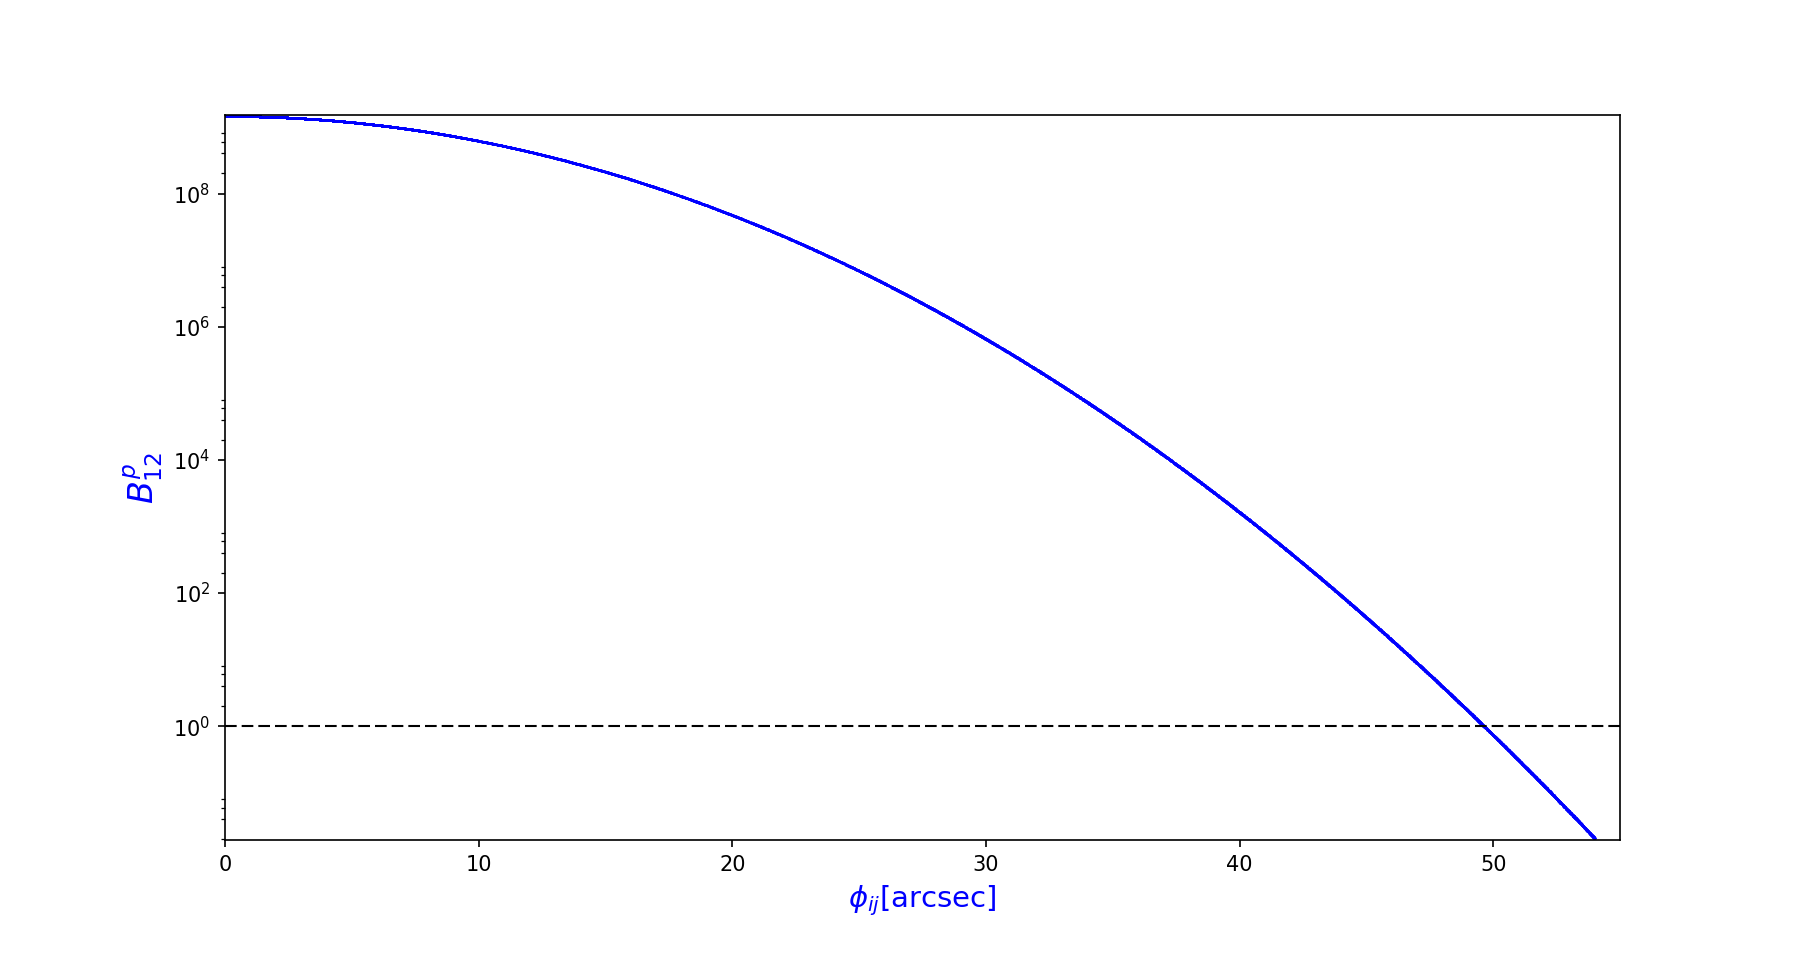
\includegraphics[width=\textwidth]{4_cross_identificacion/matching_ghbayes_posmatching_gh.png}
    \end{center}
    \vspace*{-10mm}
    \caption{\small Representación del factor de Bayes posicional en función de la distancia angular para las contrapartidas formadas por observaciones pertenecientes a \hatlas\ que se encuentran a una distancia angular inferior a \maths{54\:\mathrm{arcsec}} de otra perteneciente a \gama. La línea horizontal discontinua separa las contrapartidas con valores \maths{B^{p}_{12}<1} y \maths{B^{p}_{12}>1}. Considerando los valores de los errores instrumentales del catálogo \gama, \maths{\sigma_g^{p}\simeq0.297\;\mathrm{arcsec}} y del catálogo \hatlas,  \maths{\sigma_h^{p}\simeq7.63\;\mathrm{arcsec}}, el valor máximo que puede tomar \maths{B^{p}_{12}~\!\!~=~\!\!~9~\times~10^{9}} y la separación angular para la cual \maths{B^{p}_{12}=1} es \maths{\phi_{12}\sim49.64\:\mathrm{arcsec}}.}
    \label{fig:bayes_posicional}
\end{figure}

\vspace{-5mm}

\begin{figure}[H]
    \begin{center}
         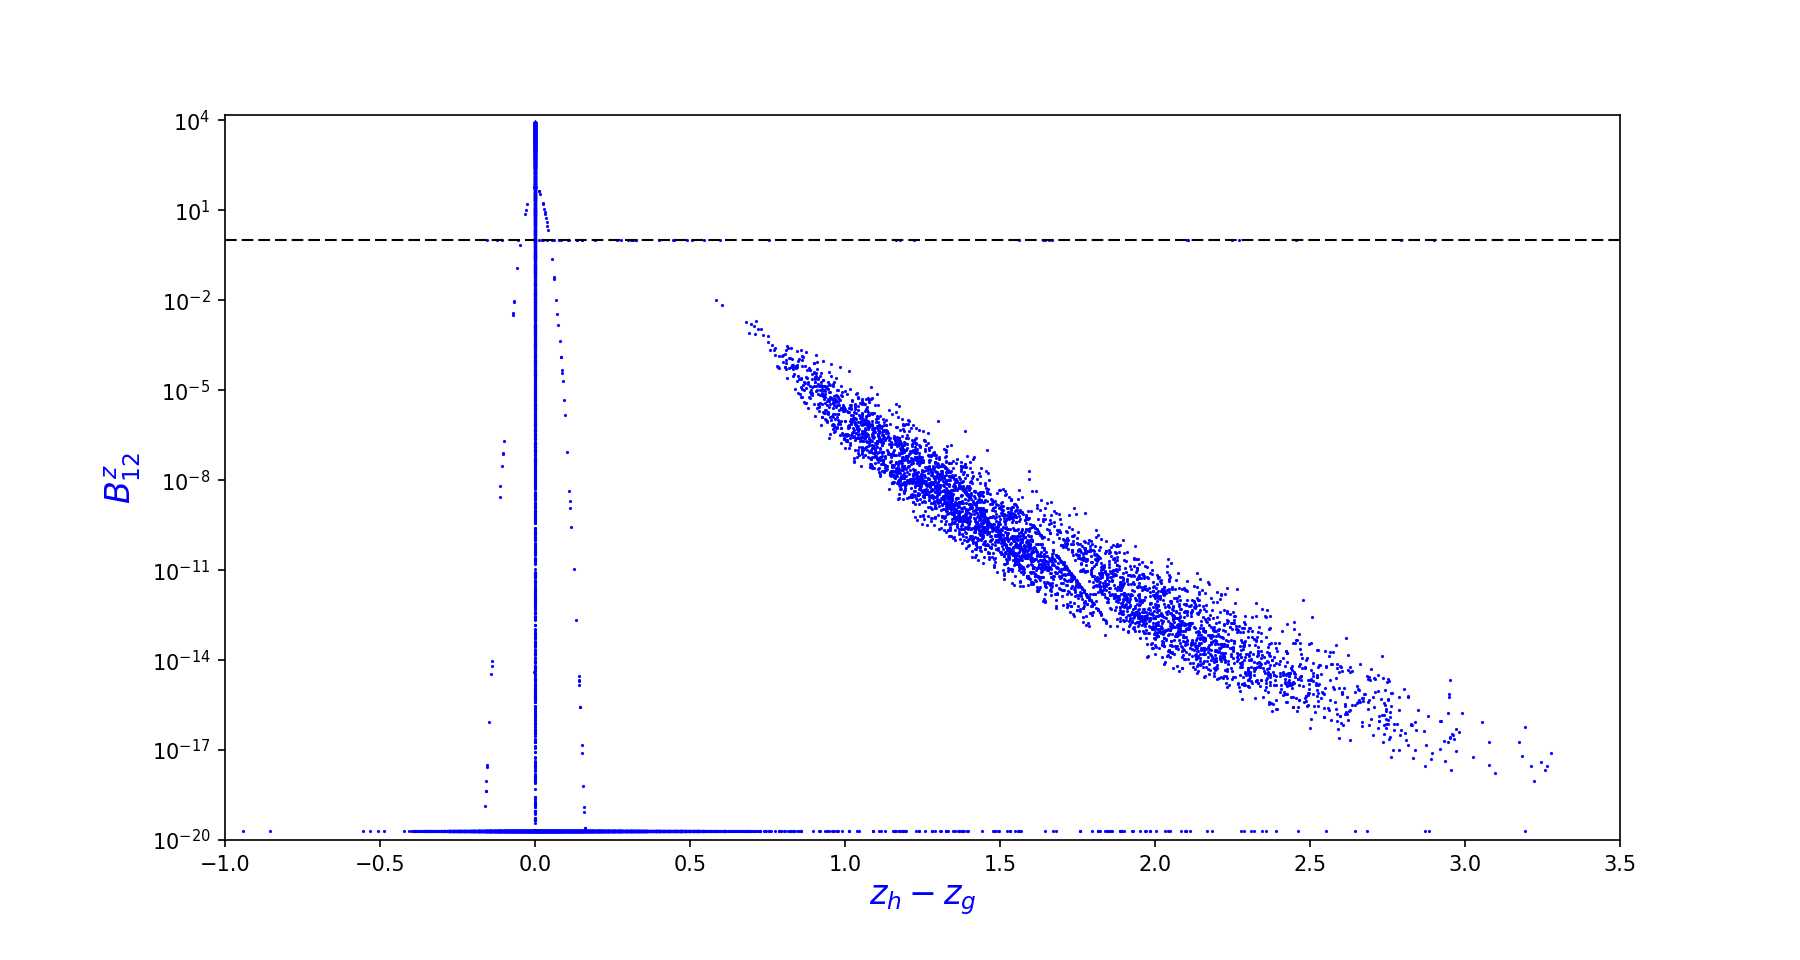
\includegraphics[width=\textwidth]{4_cross_identificacion/matching_ghbayes_zmatching_gh.png}
    \end{center}
    \vspace*{-10mm}
    \caption{\small Representación del factor de Bayes fotométrico en función de la diferencia entre los \rt\ de los catálogos \hatlas\ y \gama,  \maths{z_h-z_g}, para todas las contrapartidas formadas por observaciones de \hatlas\ que se encuentran a una distancia angular inferior a \maths{54\:\mathrm{arcsec}} de otra de \gama\ tomando \maths{z_{max}=3.5}. La línea discontinua horizontal marca el límite entre los puntos con valores \maths{B^{z}_{12}<1} y \maths{B^{z}_{12}>1}. En este caso, a diferencia del factor de Bayes posicional, cada medida del \rt\ tiene su propio valor del error, por lo que al realizar la representación los puntos aparecen como una nube de puntos. El valor máximo que puede tomar el factor de Bayes espectroscópico es \maths{B^{z}_{12}=8462} considerando \maths{z_h-z_g=0} y \maths{\sigma^z=1.1\times{10}^{-4}} para las dos observaciones que forman el pareo.}
    \label{fig:bayes_fotométrico}
\end{figure}


\subsection{Factor de Bayes posicional propuesto por Budavári \& Szalay}\label{sec:bayes_posicional}

Estos autores modelizan la posición verdadera de un objeto sobre la esfera celeste mediante un vector tridimensional unitario \maths{\boldsymbol{m}} y las posiciones observadas del mismo a partir del conjunto de vectores unitarios  \maths{D=\{\boldsymbol{x}_1,\boldsymbol{x}_2\ldots \boldsymbol{x}_n\}}. 
Debido a que hay un error instrumental, no podemos afirmar que la medida sobre la posición de un objeto, \maths{{\boldsymbol{x}}_i}, se corresponda exactamente con su posición verdadera \maths{\boldsymbol{m}}; por ese motivo se describe de forma estadística su posición a través de una función densidad de probabilidad (PDF), \maths{p(\boldsymbol{x}|\boldsymbol{m},H_k)}, que nos proporciona la probabilidad de que la verdadera posición del objeto sea \maths{\boldsymbol{m}} partiendo de la medida \maths{\boldsymbol{x}}. Estos autores hacen la propuesta de modelizar la PDF a través de una función gaussiana tridimensional normalizada\footnote{En la Sección~\ref{sec:bayes_posicional} y la Sección~\ref{sec:bayes_fotometrico} se ha simplificado la notación con respecto al resto del documento para evitar posible confusiones con las potencias. En esta sección, \maths{\sigma} es equivalente a lo que en el resto de la memoria denominamos \maths{\sigma^{z}} y en la siguiente, \maths{\sigma} equivale a \maths{\sigma^{p}}.}, 

\begin{equation*}
    p(\boldsymbol{x}|\boldsymbol{m},H_k)=N(\boldsymbol{x}|\boldsymbol{m})=\frac{w \delta (\left|\boldsymbol{x_1} \right|-1)}{4\pi \sinh{w}} \exp{(w \boldsymbol{x}\cdot \boldsymbol{m})},
\end{equation*}

con \maths{w=1/{\sigma}^{2}} y la \cultismo{probabilidad a priori} \maths{P(\boldsymbol{m}|H_k)}, como una delta de Dirac\footnote{Se trata de una distribución no informativa, es decir, la probabilidad se reparte por igual en todo el espacio paramétrico.},

\begin{equation}\label{eq:delta}
    p(\boldsymbol{m}|H_k)=\frac{1}{4\pi} \delta (\left|\boldsymbol{m} \right|-1).
\end{equation}

El factor de Bayes se obtiene a partir del cociente de las funciones verosimilitud (Definición~\ref{def:factor_bayes}),

\begin{equation}\label{eq:f_bayes_posicional}
    B^{p}_{12}=\frac{p(D|H_1)}{p(D|H_2)}.
\end{equation}

En el caso de que se cumpla la hipótesis \maths{H_1}, el conjunto de medidas \maths{D}, hará referencia a una única posición \maths{\boldsymbol{m}}. Debido a que cada medida \maths{\boldsymbol{x}_i} tiene su su propia PDF \maths{p_i(\boldsymbol{x}_i|\boldsymbol{m},H_1)}, la PDF conjunta, \maths{p(D|\boldsymbol{m},H_1)}, se expresa como el producto de las PDFs independientes,

\begin{equation*}
    p(D|\boldsymbol{m},H_1)=\prod_{i=1}^{n} p_i({\boldsymbol{x}}_i|\boldsymbol{m})=\prod_{i=1}^{n}N({\boldsymbol{x}}_i|\boldsymbol{m})=\prod_{i=1}^{n}\frac{w_i \delta (\left|{\boldsymbol{x}}_i \right|-1)}{4\pi \sinh{w_i}} \exp{(w_i {\boldsymbol{x}}_i\cdot \boldsymbol{m})}
\end{equation*}

y la función verosimilitud \maths{ p(D|H_1)} resulta ser

\vspace{-4mm}

\begin{multline*}
    p(D|H_1)=\int p(\boldsymbol{m}|H_1)\,p(D|\boldsymbol{m},H_1)\,d^3m
    =\\
    \int \frac{\delta (\left|\boldsymbol{m} \right|-1)}{4\pi}\,\prod_{i=1}^{n} \frac{w_{i} \;\delta (\left|\boldsymbol{x}_{i} \right|-1)}{4\pi \sinh{w_{i}}} \exp{\left(w_{i}\boldsymbol{x}_{i}\cdot \boldsymbol{m}\right)}\,d^3m
    = \\
    \left[ \prod_{i=1}^{n} \frac{w_{i} \;\delta (\left|\boldsymbol{x}_{i} \right|-1)}{4\pi \sinh{w_{i}}} \right] \int{\frac{\delta (\left|\boldsymbol{m} \right|-1)}{4\pi}} \exp{ \left(\sum_{i=1}^{n}{w_{i}{\boldsymbol{x}}_{i}\cdot \boldsymbol{m}}\right)}\,d^3m.
\end{multline*}

Introduciendo

\begin{equation*}
    w\boldsymbol{x}=\sum_{i=1}^{n}w_i\boldsymbol{x}_i
\end{equation*}

y multiplicando y dividiendo por \maths{\frac{\sinh w}{w}}, tenemos que

\begin{multline*}
    p(D|H_1)=\left[\frac{\sinh w}{w}\prod_{i=1}^{n} \frac{w_{i} \;\delta (\left|\boldsymbol{x}_{i} \right|-1)}{4\pi \sinh{w_i}}\right] \int{\frac{w \delta (\left|\boldsymbol{m} \right|-1)}{4\pi\sinh{w}}} \exp{ \left(w \boldsymbol{x}\cdot \boldsymbol{m}\right)}\,d^3m
    =\\
    \frac{\sinh{w}}{w}\prod_{i=1}^{n}\frac{w_i}{\sinh{w_i}}\frac{\delta (\left|\boldsymbol{x}_i \right|-1)}{4\pi}.
\end{multline*}

Por otra parte, la hipótesis alternativa \maths{H_2}, representa la hipótesis de que las medidas realizadas son pertenecientes a los objetos diferentes, por tanto el conjunto de medidas \maths{D=\{\boldsymbol{x}_1,\boldsymbol{x}_2\ldots \boldsymbol{x}_n\}} hace referencia al conjunto de posiciones verdaderas \maths{\{\boldsymbol{m}_1,\boldsymbol{m}_2\ldots \boldsymbol{m}_n\}}. y la función verosimilitud de la hipótesis \maths{H_2},

\begin{multline*}
    p(D|H_2)= \prod_{i=1}^{n} \left[ \int{p\left( \boldsymbol{m_i} | H_2 \right)  p_i\left(\boldsymbol{x}_i |\boldsymbol{m}_i,H_2 \right)\,\mathrm{d}^3m_i} \right]=\\
    \prod_{i=1}^{n} \int \frac{\delta (\left|\boldsymbol{m}_i \right|-1)}{4\pi} \frac{w_i \delta (\left|\boldsymbol{x}_i \right|-1)}{4\pi \sinh{w_i}} \exp{\left(w_i\boldsymbol{x}_i\boldsymbol{m}_i\right)}\,d^3m_i =\prod_{i=1}^{n}\frac{\delta (\left|\boldsymbol{x}_i \right|-1)}{4\pi}.
\end{multline*}

Al sustituir en la Ecuación~\ref{eq:f_bayes_posicional} obtenemos,

\begin{equation*}
    B_{12}^{p}=\frac{p(D|H_1)}{p(D|H_2)}= \frac{\sinh{w}}{w}\prod_{i=1}^{n}\frac{w_i}{\sinh{w_i}}
\end{equation*}

que se aproxima a

\begin{equation*}
    B_{12}^{p}=
    {2}^{(n-1)}\frac{{\prod_{i=1}^{n}{w_i}}}{ \sum_{i=1}^{n}{w_i}}\exp{\left(- \frac{ \sum_{i<j}{w_i w_j {{\phi}_{ij}}^{2}} }{2\sum_{i=1}^{n}{w_i}} \right)}
\end{equation*}

y para dos catálogos astronómicos, se reduce a

\begin{equation}\label{eq:bayes_posicional}
    B_{12}^{p}= \frac{2}{{\sigma}^2_1+{\sigma}^2_2}\exp{\left(- \frac{{\phi}^{2}_{12}}{2({\sigma}^2_1+{\sigma}^2_2)} \right)}
\end{equation}

como expresión final para el factor de Bayes posicional.

\subsection{Factor de Bayes fotométrico propuesto por Budavári}\label{sec:bayes_fotometrico}

A diferencia del factor de Bayes posicional en que que se resolvía el problema para un caso general, aquí se va resolver el caso en el que se dispone de dos catálogos. Ahora, el valor verdadero del \rt\ de un objeto viene representado por \maths{\tau} y el conjunto de medidas se reduce a \maths{D=\{z_1,z_2\}}. De nuevo, debido a que existe una incertidumbre asociada a estas medidas, el valor medido no se corresponde exactamente con el valor real por lo que hay que proponer una PDF. En este caso se elige la función gaussiana unidimensional normalizada de la forma

\begin{equation*}
    p(z|\tau,H_{k})=N(z|\tau)=\frac{1}{\sqrt{2\pi}\sigma}\exp{\left( - \frac{{\left(z-\tau \right)}^{2}}{2{\sigma}^{2}}\right)}
\end{equation*}

y una \cultismo{probabilidad a priori} constante entre 0 y un valor máximo \maths{z_{max}},

\begin{equation*}
    p(\tau|{H}_{k})=p_0,
\end{equation*}

cuyo valor viene dado por la condición de normalización

\begin{equation*}
    \int_0^{z_{max}}p(\tau|{H}_{k})\:\mathrm{d}\tau=1 \implies p_0=\frac{1}{z_{max}}.
\end{equation*}

En caso de que ambas medidas se correspondan a único valor, la densidad de probabilidad conjunta se expresa como

\begin{equation*}
    p(D|\tau,{H}_{1})=\prod_{i=1}^{2} p_i(z_i|\tau,H_{1})=\prod_{i=1}^{2} N(z_i|\tau) =\frac{1}{2\pi{\sigma}_{1}{\sigma}_{2}}\exp{\left(-\frac{{(\tau-z_1)}^{2}}{2{\sigma}_{1}^{2}}-\frac{{(\tau-{z}_{2})}^{2}}{2{\sigma}_{2}^{2}}\right)}
\end{equation*}

y la función verosimilitud para la hipótesis \maths{H_1} será

\begin{multline*}
    p(D|{H}_{1})=\int_{0}^{z_{max}} p(\tau|{H}_{1})p(D|\tau,{H}_{1}) \mathrm{d}\tau=\\
    \resizebox{.9\hsize}{!}{$\frac{p_0}{2\sqrt{2\pi}\sqrt{{\sigma}_{1}^2+{\sigma}_{1}^2}}\exp{\left(-\frac{{(z_1-z_2)}^{2}}{2({\sigma}_{1}^{2}+{\sigma}_{2}^{2})}\right)}\left[ \erf{\left( \frac{{\sigma}_{1}^{2}z_2+{\sigma}_{2}^{2}z_1}{\sqrt{2}\sigma_1\sigma_2\sqrt{\sigma_1^2+\sigma_2^2}}  \right)}- \erf{\left( \frac{{\sigma}_{1}^{2}(z_2-z_{max})+\sigma_2^2(z_1-z_{max})}{\sqrt{2}\sigma_1\sigma_2\sqrt{\sigma_1^2+\sigma_2^2}}  \right)} \right]$}.
\end{multline*}

Por otro lado, si las dos medidas pertenecen a dos objetos diferentes, la función verosimilitud se obtiene a partir de

\begin{multline*}
    p(D|H_2)=\prod_{i=1}^{2}\left[\int_{0}^{z_{max}} p({\tau}_{i}|H_2){p}_{i}(z_i|{\tau}_{i},H_2)\:\mathrm{d}{\tau}_{i} \right]=\\
    \frac{p_0^2}{4}\left[\erf{\left(\frac{z_1}{\sqrt{2}\sigma_1}\right)}-\erf{\left(\frac{z_1-z_{max}}{\sqrt{2}\sigma_1}\right)}\right]\left[\erf{\left(\frac{z_2}{\sqrt{2}\sigma_2} \right)}-\erf{\left(\frac{z_2-z_{max}}{\sqrt{2}\sigma_2} \right)}\right].
\end{multline*}

Sustituyendo las expresiones obtenidas para las funciones verosimilitud en la definición del factor de Bayes~\ref{def:factor_bayes}, tenemos la expresión que se va a utilizar en este trabajo,

\begin{equation}\label{eq:factor_bayes_fotometrico}
    B_{12}^{z}=\frac{\sqrt{2}\:z_{max}\exp{\left(-\frac{{(z_1-z_2)}^{2}}{2({\sigma}_{1}^{2}+{\sigma}_{2}^{2})}\right)}\left[ \erf{\left( \frac{{\sigma}_{1}^{2}z_2+{\sigma}_{2}^{2}z_1}{\sqrt{2}\sigma_1\sigma_2\sqrt{\sigma_1^2+\sigma_2^2}}  \right)}- \erf{\left( \frac{{\sigma}_{1}^{2}(z_2-z_{max})+\sigma_2^2(z_1-z_{max})}{\sqrt{2}\sigma_1\sigma_2\sqrt{\sigma_1^2+\sigma_2^2}}  \right)} \right]}{\sqrt{\pi(\sigma_1^2+\sigma_2^2)}\left[\erf{\left(\frac{z_1}{\sqrt{2}\sigma_1}\right)}-\erf{\left(\frac{z_1-z_{max}}{\sqrt{2}\sigma_1}\right)}\right]\left[\erf{\left(\frac{z_2}{\sqrt{2}\sigma_2} \right)}-\erf{\left(\frac{z_2-z_{max}}{\sqrt{2}\sigma_2} \right)}\right]}.
\end{equation}

para el factor de Bayes fotométrico\footnote{Cuando realicemos los cálculos vamos a asumir que \maths{z_1\geq0}, \maths{z_2\geq0}, \maths{\sigma_1>0}, \maths{\sigma_2>0}, \maths{z_{max}>0} y \maths{z_{max}>z_1\land z_2}}. Si consideramos que las medidas del \rt\ de uno de los catálogos no tienen error (por ejemplo si la medida es espectroscópica), \maths{\sigma_2=0} y la Ecuación~\ref{eq:factor_bayes_fotometrico} se reduce a

\begin{equation*}
    B_{12}^{z}=\frac{\sqrt{\frac{2}{\pi}}z_{max}\exp{\left(-\frac{{(z_1-z_2)}^{2}}{2{\sigma_1}^2}\right)}}{\sigma_1 \left( \erf{(\frac{z_1}{\sqrt{2}\sigma_1})}-\erf{(\frac{z_1-z_{max}}{\sqrt{2}\sigma_1})} \right)}.
\end{equation*}

En el límite en el que \maths{z_{max}\gg z_1 \gg \sigma} el paréntesis del denominador que contiene las funciones error tiende a \maths{1-(-1)=2} y se obtiene la ecuación:

\begin{equation*}
    B_{12}^{z}=\frac{z_{max}}{\sqrt{2\pi\sigma_1}}\exp{\left(-\frac{{(z_1-z_2)}^{2}}{2{\sigma_1}^2}\right)}
\end{equation*}

que encontramos en \cite{tesis:alberto_manjon}.